\documentclass[a4paper,12pt]{report}
%%%%%%%%%%%%%%%%%%%%%%%%%%%%%%%%%%%%%%%%%%%%%%%%%%%%%%%%%%%%%%%%%%%%%%%%%
%%%%%% Definizioni:
\def\titolotesi{Implementazione di un sistema mobile ed autonomo per la ricerca di oggetti in base al colore} % INSERIRE TIOLO DELLA TESI
\def\laureando{Simone Mariotti}       % INSERTIRE NOME COGNOME LAUREANDO
\def\annoaccademico{2013-2014}    % INSERIRE ANNO ACCADEMICO
\def\dedica{TODO: DEDICA}      % INSERIRE DEDICA
\title{\begin{large}\textbf{\titolotesi}\end{large}}
\author{\laureando}
%%%%%% File previsti in input:
%% introduzione.tex    (deve contenere solo il testo, senza \chapter{})
%% capitolo1.tex       (deve iniziare con \chapter{titolo capitolo})
%% capitolo2.tex                           "
%% capitolo3.tex                           "
%% capitolo4.tex                           "
%% conclusioni.tex     (deve contenere solo il testo, senza \chapter{})
%% appendice.tex       (deve contenere solo il testo, senza \chapter{})
%%%%%%%%%%%%%%%%%%%%%%%%%%%%%%%%%%%%%%%%%%%%%%%%%%%%%%%%%%%%%%%%%%%%%%%%%

% Title Page

\usepackage[utf8]{inputenc}
\usepackage[italian]{babel}
\usepackage{fancyhdr}

%\usepackage[hidelinks]{hyperref}
\usepackage{hyperref}

\usepackage{epsfig}
\addto\captionsitalian{%
  \renewcommand{\listfigurename}{Elenco delle immagini}%  
}

\pagenumbering{Roman}
%\usepackage{setspace}
\newlength\sinistra
\newlength\corpo
\newlength\pagina
\setlength {\pagina} {21cm}
\setlength {\sinistra} {1.46cm}
\setlength {\corpo} {13.5cm}
\textwidth \the\corpo
\hoffset \the\sinistra
\paperwidth \the\pagina
\linespread{1.6}


\begin{document}
\begin{titlepage}
\begin{center}
\textsc{\Large Universit\`a degli Studi di Perugia}\medskip\\

{\Large Facolt\`a di Scienze Matematiche, Fisiche e Naturali}\medskip\\

\rule{10mm}{0.01mm}\medskip\\

{\small \textsc{Corso di Laurea in Informatica}}\medskip\\

\vspace*{5mm}


\includegraphics[scale=0.2]{immagini/logouni.png}

\Large Tesi di Laurea \par\bigskip

{\large \bf \titolotesi \par}

\bigskip\bigskip

\end{center}\par

\hspace{0.5cm}Laureando\hspace{7.3cm}Relatori\par

\hspace{0.0cm}\emph{\laureando}\hfill\emph{Prof.~Marco Baioletti}\\
\ \ \hspace*{3.0cm}\hfill\emph{Dott.~Emanuele Palazzetti}\\

\begin{center}

\rule{40mm}{0.01mm}\\

Anno Accademico \annoaccademico

\end{center}

\end{titlepage}

%%%% DEDICA
\newpage
\thispagestyle{empty}
\vspace*{2.5cm}
\begin{flushright}
\begin{Large}\emph{\dedica}\end{Large}
\end{flushright}
\frenchspacing
%%%%%% Ringraziamenti (opzionale)
%
%\chapter*{Ringraziamenti}
%Voglio ringraziare ....
%%%%%%%%%%%%%%%%%%%%%%%%%%%%%%%%%

%%%% INDICE
\thispagestyle{empty}
\tableofcontents



\fancyhf{}
\pagestyle{fancy}
%%%% fine prologo

%%%% Inizio corpo tesi

%%%% Introduzione  
\newpage
\pagenumbering{arabic}
%!TEX root = Tesi__Simone_Mariotti.tex
\chapter*{Introduzione}
\addcontentsline{toc}{chapter}{Introduzione}
\section* {Obiettivi}
\section* {Strumenti utilizzati}
        %Il testo dell'introduzione e' in un file esterno: "introduzione.tex"



%%%% CAPITOLI
%\chapter{Titolo capitolo primo}                 %%% OGNI CAPITOLO INIZIERA' CON QUESTE DUE ISTRUZIONI!
%\fancyhead[RO]{\bfseries Titolo capitolo primo} %%%

%!TEX root = Tesi__Simone_Mariotti.tex
\chapter{Visione Artificiale}
\fancyhead[R]{\bfseries Visione Artificiale} 	 	
\fancyfoot[C]{\thepage } 
La \textit{visione artificiale} ha come compito la creazione di 
un modello del mondo reale in tre dimensioni a partire da numerose 
immagini bidimensionali per cercare di emulare il processo biologico della vista.
Negli esseri umani, così come in molte altre specie, vedere non è solo scattare una 
fotografia bidimensionale mentale di un ambiente, ma è interpretare le informazioni
ricevute attraverso la retina per analizzare e creare un modello 3D dell'ambiente
circostante.\\	
Un sistema di visione artificiale, per provare ad avvicinarsi alla capacità visiva
e di interpretazione umana, ha bisogno di numerosi componenti di diversa natura: 
ottici, elettronici e meccanici per acquisire e memorizzare le immagini da elaborare.
Il primo tentativo in tal senso è datato 1883 quando  Paul Gottlieb Nipkow 
inventò il primo sistema in grado di trasformare informazioni visive in un segnale elettrico.\cite{Nipkow1} 
\\Il sistema si basa su un disco con dei fori praticati lungo una spirale che parte dal centro del disco
e procede verso l'esterno. Il disco ruota ad una velocità costante mentre l'immagine 
inquadrata viene focalizzata da una lente verso i fori in modo che un sensore, 
posto sul retro del disco, possa percepire i cambi di luminosità della porzione di scena
inquadrata e convertire questa variazione in segnali elettrici. 
\\Il ricevitore emetterà luce in base a dei 
segnali elettrici e attraverso un disco identico al primo e in rotazione sincrona 
proietterà un'immagine con tante righe quante sono i fori del disco.\cite{Nipkow2} 
Questo sistema porterà alla creazione della TV meccanica nel 1925.
\begin{figure}[!htb] \center
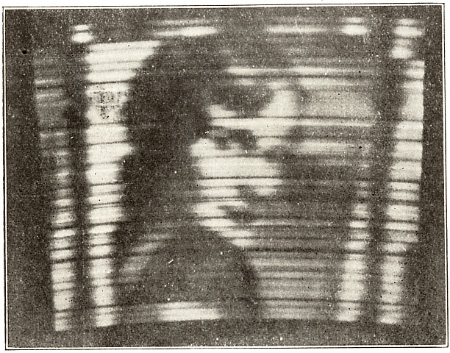
\includegraphics[width=\textwidth]{immagini/tv_meccanica.png}
\caption{Immagine visibile su una TV meccanica del 1925} 
\end{figure}
Negli anni successivi, con l'introduzione della miniaturizzazione nell'elettronica, 
sono stati compiuti enormi progressi. Da un punto di vista teorico, gli scienziati 
cominciarono ad ispirarsi al corpo umano nel tentativo di riprodurre il suo comportamento. Analizzando da vicino
l'occhio e in particolare la retina hanno scoperto che era formata da minuscoli 
recettori sensibili alla luce collegati al cervello tramite il nervo ottico. 
Si è così deciso di creare dei 
micro sensori di luce e formarne un'enorme matrice. Il primo risultato di questi studi 
si ebbe circa 40 anni dopo e fu il sensore CCD\footnote{Charge-Coupled Device.}, 
ideato da Willard S. Boyle e George E. Smith nel 1969 presso i Bell Laboratories,
mentre dobbiamo aspettare il 1993 per vedere i primi prototipi funzionanti del 
sensore CMOS\footnote{Complementary Metal-Oxide-Semiconductor.} sviluppati presso 
il Jet Propulsion Laboratory, entrambi hanno come elemento base il fotodiodo che 
equivale ad un pixel. Il CCD è un sensore 
analogico\footnote{Il sensore più grande esistente è di 1,4 Gigapixel ed è 
montato sul telescopio Pan-STARRS sviluppato per l'individuazione di meteoriti in
 rotta di collisione con la Terra.} che ha bisogno di più energia 
ma offre in genere una qualità superiore un rumore minore ad un costo più elevato.\\
\begin{figure}[!htb] \center
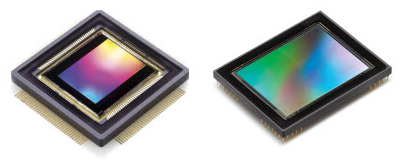
\includegraphics[scale=0.8]{immagini/ccd-cmos.png}
\caption{Due sensori moderni. A sinistra un sensore CMOS a destra uno CCD} 
\end{figure}
Il CMOS è un sensore digitale che offre una buona qualità di immagine ad costo minore;
per contro l'immagine presenta un forte rumore a causa della conversione 
analogico-digitale.\\
La visione artificiale ha principalmente tre utilizzi:
\begin{itemize}
\item \textbf{Ricognizione:} ricercare uno o più oggetti, scelti a priori, e organizzarli in 
insiemi generici o classi mantenendo informazioni riguardo il loro posizionamento 
nella scena. \\Esempio: ricercare in un'immagine o in un video tutte le persone, 
le macchine o gli animali. 
\item \textbf{Identificazione:} identificare una istanza specifica di una classe 
di oggetti. \\Esempio: ricercare in un'immagine o in un video un volto, 
una macchina o un animale specifico.. 
\item \textbf{Individuazione:} cercare una condizione specifica nell'immagine. 
\\Esempio: cercare imperfezioni nelle immagini a raggi X di superfici o materiali.
\end{itemize}
Un campo che ne fa massiccio utilizzo è la modellazione di ambienti 3D a partire 
da due o più immagini 2D; questo è stato reso possibile 
grazie all'enorme aumento della capacità di elaborazione grafica delle GPU.\\
La visione artificiale è stata applicata a molti altri campi nei quali si è verificata 
una vera e propria rivoluzione.

Uno di questi è la medicina nella quale l'introduzione di questa tecnica ha portato
all'analisi di radiografie, angiografie,
tomografie e altre immagini mediche. In questo modo è possibile identificare anomalie e 
problemi, quali i tumori, che non sarebbero visibili all'occhio umano 
se non in seguito a procedure molto invasive.

Un altro campo è quello del controllo di veicoli autonomi i quali stanno aumentando
ad un ritmo vertiginoso, progressivamente al migliorarsi delle tecniche di 
visione artificiale. Autovetture, droni, robot e carri per il rifornimento 
sono solo degli esempi a cosa può portare la visione artificiale applicata nei settori 
civili e di ricerca.
\begin{figure}[!htb] \center
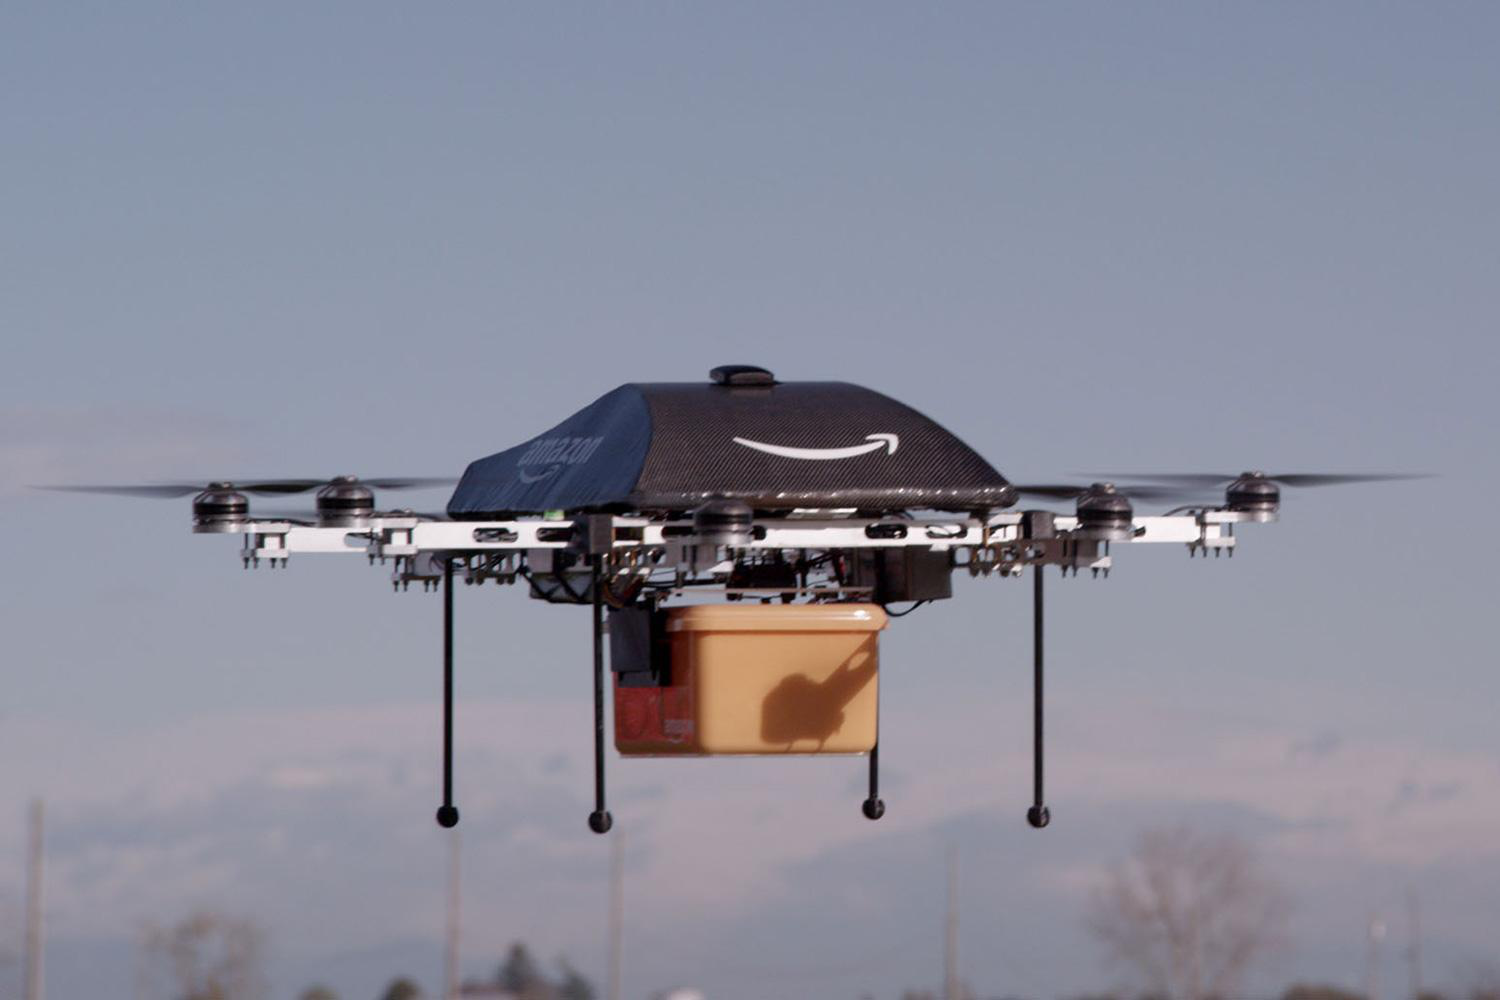
\includegraphics[scale=0.2]{immagini/amazon-air.png}
\caption{Drone della società statunitense Amazon. Consegnerà prodotti a domicilio in completa autonomia} 
\end{figure}
La nostra tesi si concentra proprio sull'applicazione ad un robot autonomo dei 
concetti di visione artificiale appena descritti.


%!TEX root = Tesi__Simone_Mariotti.tex
\chapter{Componenti del robot}
\section{Hardware}
\subsection{UDOO Quad}
UDOO è un progetto tutto italiano di una piattaforma hardware destinata alla 
generazione dei ``makers'', cioè quelle persone che vogliono realizzare i 
proprie progetti con le tecnologia a basso costo ad oggi disponibili. La 
scheda ha visto la luce dopo una sorprendente campagna di crowdfunding
\footnote{dall'inglese crowd, folla e funding, finanziamento. In italiano finanziamento collettivo.} terminata l'8 Giugno 2013 con 4172 donazioni per un totale di \$641.612 a fronte di \$27.000 richiesti per iniziare la produzione. Per permettere l'utilizzo di librerie e applicazioni computazionalmente pesanti 
come openCV, PureData e altre UDOO monta un processore ARM Freescale i.MX6 
Cortex-A9 Quad core 1GHz che supporta sia Android che Linux. Il tutto è 
completato da una GPU Vivante, 1GB di RAM DDR3, numerose porte di I/O come 
SATA, microfono, audio out, Ethernet, HDMI, USB, connettore per display LVDS 
con touch screen, connettore CSI per camera esterna e connettività bluetooth e 
Wi-Fi. La periferica di ``boot'' è una microSD il che permette un rapido 
passaggio da Linux a Android e viceversa. Quello che però rende veramente 
unica questa piattaforma, e che ne ha fatto la nostra scelta per questo 
progetto di tesi, è la presenza di un Arduino DUE completamente integrato 
nella stessa board. 
E' presente una CPU Atmel SAM3X8E ARM Cortex-M3 \footnote{la stessa di cui 
dispone l'Arduino DUE} e 76 GPIO\footnote{General Purpose Input/Output}, di 
cui 62 digitali e 14 digitali/analogici, disposti per essere perfettamente 
compatibili con la piedinatura dell'Arduino DUE e dell'Arduino UNO Rev.3.

\begin{figure}[!htb] \center
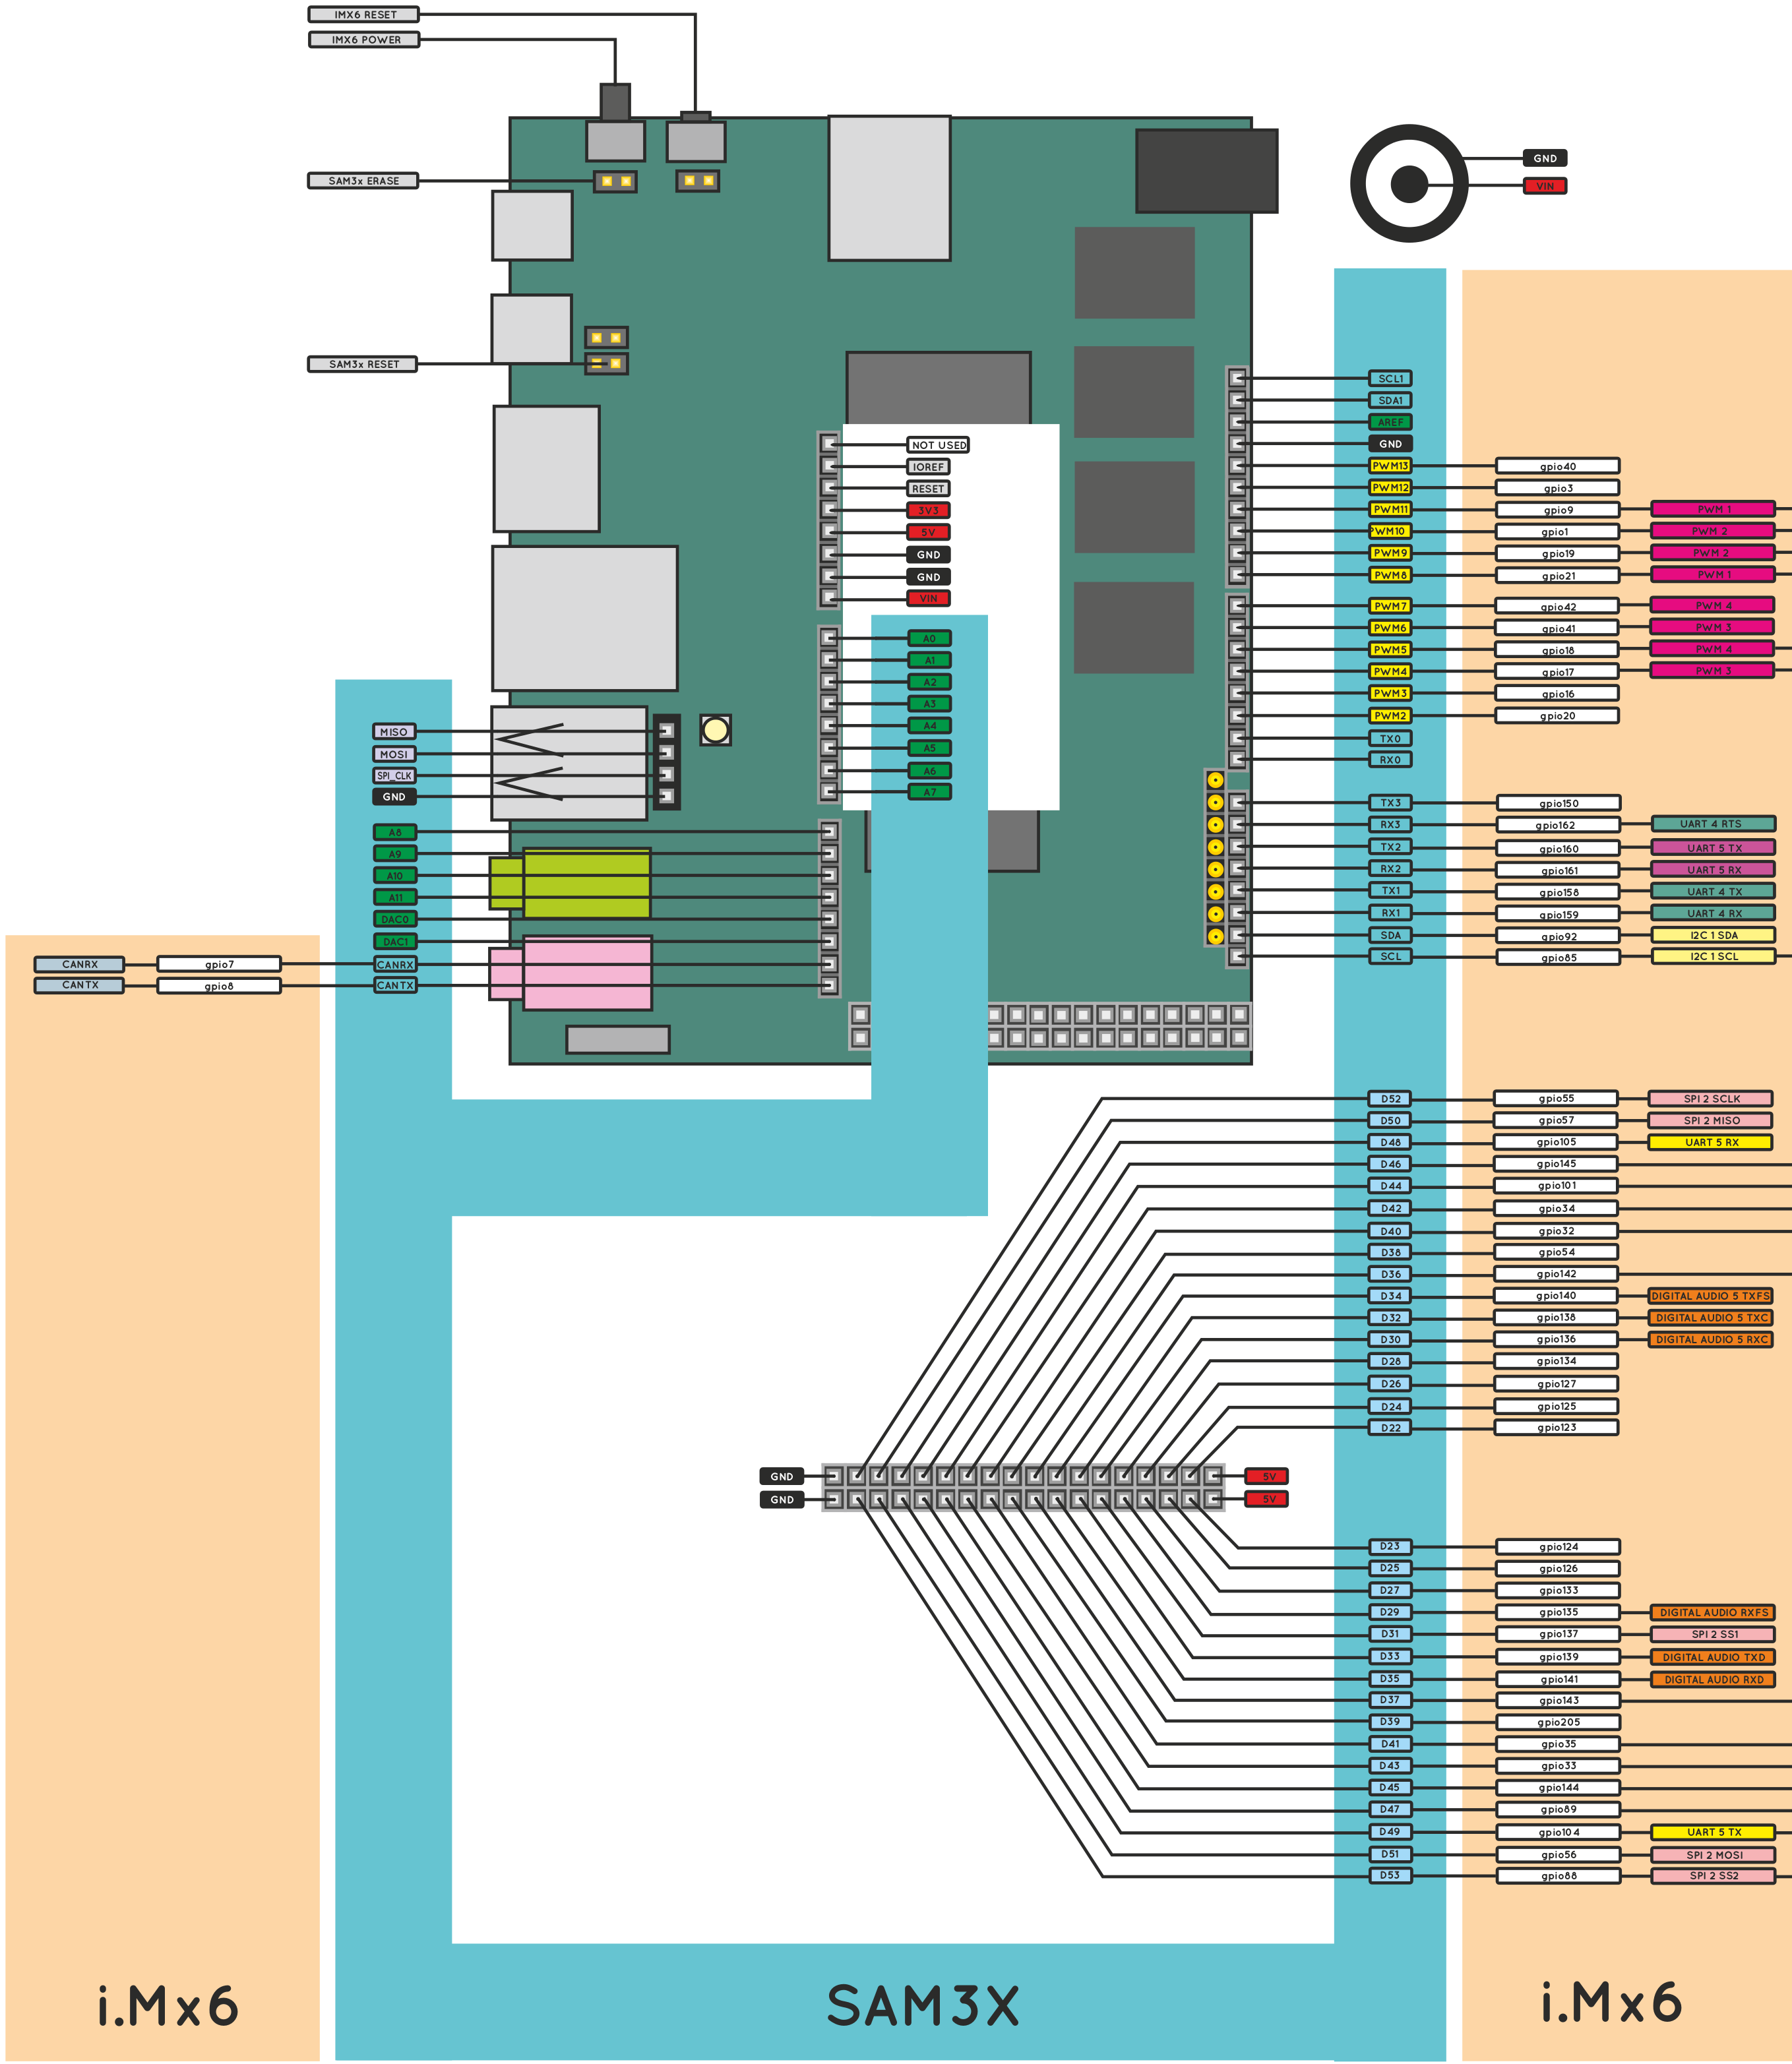
\includegraphics[width=\textwidth]{immagini/udoo_pinout.png}
\caption{Schema piedinatura UDOO} 
\end{figure}

La presenza di un Arduino DUE all'interno della board rende UDOO una scheda di 
prototipazione a tutti gli effetti e apre nuovi interessanti scenari e 
possibilità unendo la versatilità e semplicità di Arduino, la potenza di 
calcolo del Freescale i.MX6 e le numerose periferiche disponibili per Linux o 
Android.\\
Essendo una piattaforma open-source è possibile accedere alla shell del 
sistema operativo come root tramite la porta seriale integrata e modificare a 
piacimento la configurazione del sistema operativo. Arduino è collegato al 
Freescale i.MX6 tramite un bus interno e quindi viene rilevato come una 
normale periferica USB da Linux; su Android la comunicazione tra i due 
dispositivi avviene sullo stesso bus ma usa lo standard USB OTG\footnote{On-The
-Go è una specifica che permettere di agire come host ad un qualsiasi  
dispositivo (tipicamente smartphone e tablet). A differenza dell'USB classico 
l'OTG è driver-less, cioè non necessita l'installazione di driver specifici 
per ogni dispositivo}. L'interconnessione tra l'accessorio Arduino e 
l'applicazione Android è realizzata tramite l'ADK\footnote{Android Development 
Kit} 2012, di cui parleremo più avanti in questo stesso capitolo, che permette 
l'integrazione delle più disparate periferiche a dispositivi Android tramite 
una connessione USB o Bluetooth.
\subsection {Tank Kit}
Per dare la giusta stabilità e manovrabilità al robot si è deciso di usare una
 locomozione a cingoli che richiede solo due motori e permette di ruotare sul 
 posto o comunque in spazi ristretti: la nostra scelta è stata il ``Multi-
 Chassis - Tank Version''. Questa piattaforma, appositamente pensata per la 
 realizzazione di robot multifunzione, si è rivelata la scelta perfetta in 
 quanto possiede due potenti motori DC già forniti di riduttori 48:1 per 
 affrontare terreni impervi e scoscesi, quattro ruote da 52mm di diametro a 
 cui sono applicati i due cingoli.E' presente anche un alloggiamento per un 
 servomotore standard che nella nostra applicazione non è stato usato. 
 L'intelaiatura, di alluminio spesso 2,5mm, presenta numerosi fori e asole per 
 il montaggio di accessorie quali sensori, staffe e motori. Presenta inoltre 
 un ``doppio fondo'' in cui sono alloggiati i motori DC e i riduttori e in cui 
 è possibile sistemare altri componenti che non debbano essere facilmente 
 accessibili.
\subsection {Sensori}
\subsubsection{Sensore di riflessività - QRD1114}
Avevamo la necessità di fornire al robot un modo per rilevare eventuali 
sconfinamenti dall'ambiente di test che fosse il più flessibile possibile. 
Abbiamo optato per il sensore di riflessività QRD1114 prodotto dalla Fairchild 
Semiconductor: questo sensore è costituito da un LED infrarosso e un 
fototransistor tarato sulla luce infrarossa e con filtro per la luce solare 
onde evitare disturbi. Il robot era stato pensato per lavorare su un tavolo o 
altra superficie con spigoli netti: per rilevare l'imminente caduta in questo 
tipo di ambiente sarebbe stato sufficiente un sensore di distanza puntato 
verso terra. Con il sensore di riflessività abbiamo reso possibile l'utilizzo 
in terra o comunque in ambienti estesi delimitati da un recinto spesso circa 
10cm realizzato con materiale a basse riflettività come del semplice 
cartoncino nero opaco. Il sensore non fa differenza tra il cartoncino nero o 
lo spazio a fianco di un tavolo, rileva semplicemente una riflessività vicina 
allo zero. Il sensore così come fornito dal produttore non è direttamente 
utilizzabile, per far si che Arduino potesse acquisire dal sensore valori 
proporzionali alla riflessività del materiale in esame abbiamo dovuto 
realizzare un circuito elettronico di interfaccia. 
\begin{figure}[!htb] \center
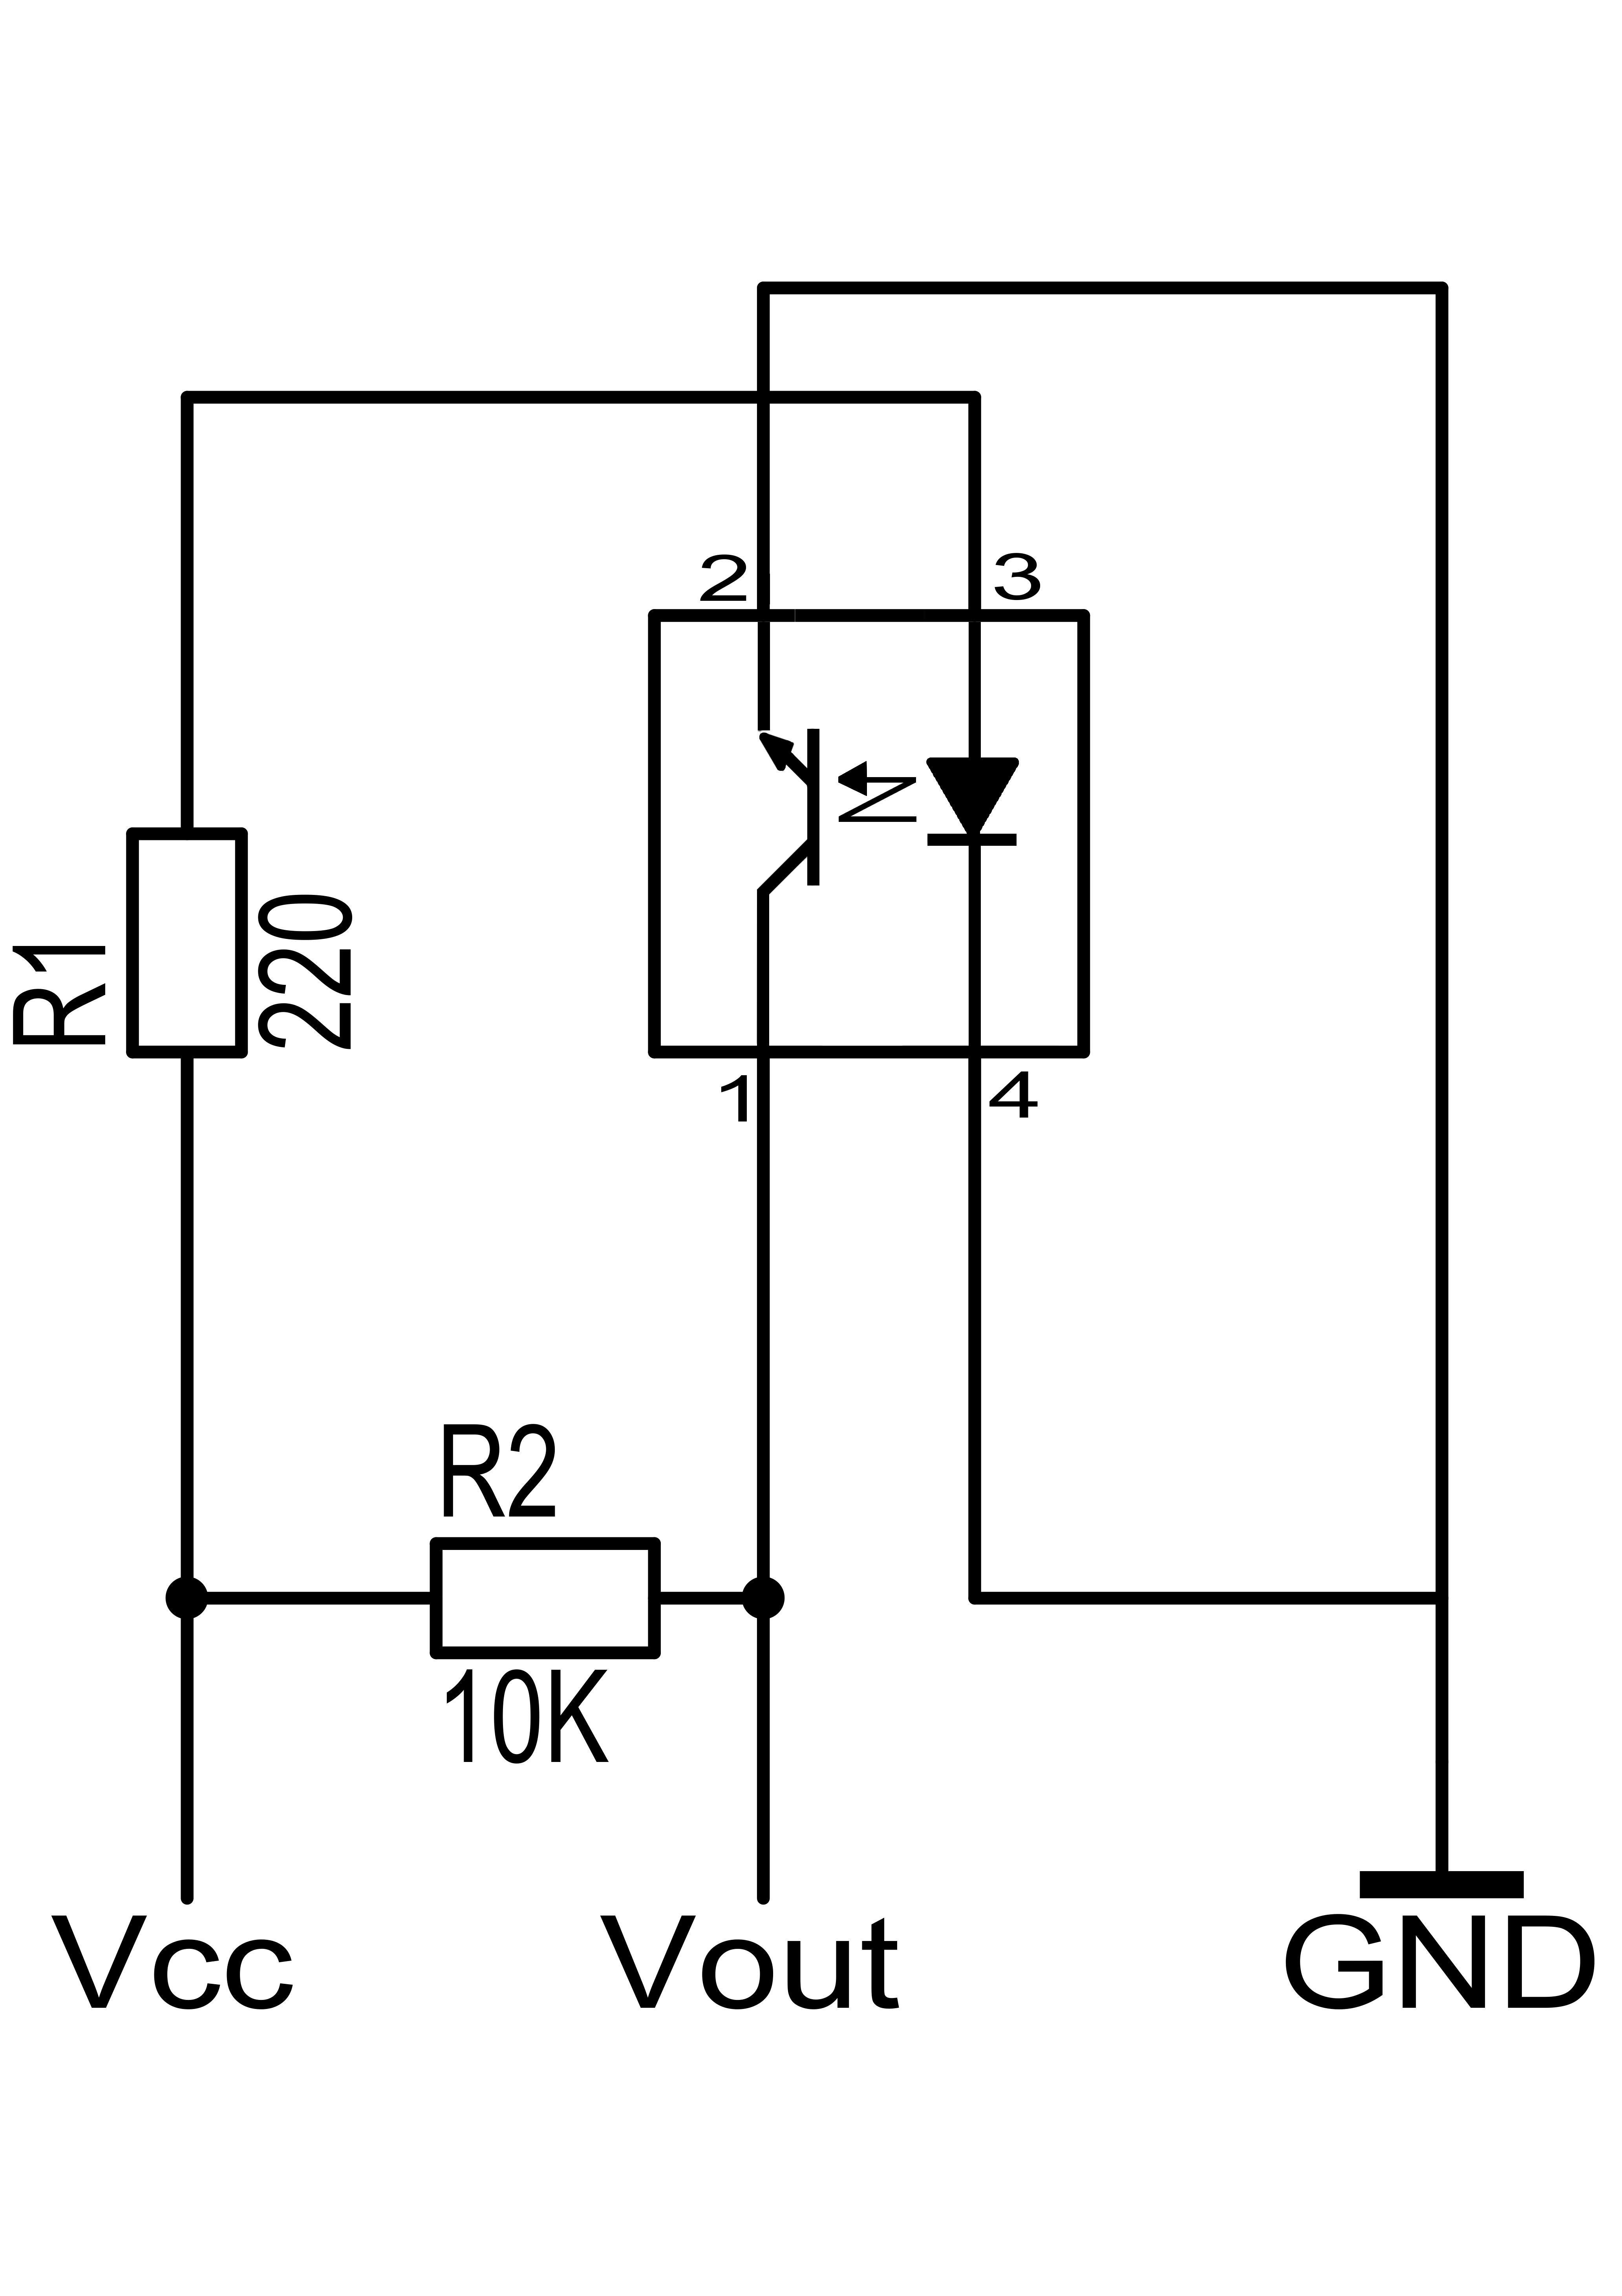
\includegraphics[ scale=0.2]{immagini/QRD1114.png}
\caption{Circuito di interfaccia tra Arduino e il sensore QRD1114} 
\end{figure}
Il circuito alimenta il LED tramite una resistenza da 220$\Omega$ (\textit{R1}) 
e collega $V_{CC}$\footnote{pari a 3,3 $V$ nell'Arduino DUE} al collettore del 
fototransistor tramite una resistenza da 10 $k\Omega$ (\textit{R2}) mentre 
l'emettitore è collegato a terra; il punto da cui prelevare il segnale ($V_{OUT
}$) è tra \textit{R2} e il collettore. Il principio alla base del circuito è 
semplice: il LED è sempre acceso e illumina in modo diffuso parallelamente al 
fototransistor. Il fototransistor in assenza di luce o, nel nostro caso, in 
presenza di una bassa riflessività si trova in stato di interdizione; i pin di 
Arduino impostati come input sono in configurazione ``alta impedenza'', 
equivalenti ad un interruttore aperto dal punto di vista circuitale, quindi 
non c'è passaggio di corrente né tramite il transistor né tramite la 
resistenza \textit{R2} il che porta esattamente il valore di $V_{cc}$ in 
ingresso ad Arduino. Quando il fototransistor è totalmente illuminato, cioè in 
presenza di alta riflessività, entra in stato di conduzione così che nel punto 
$V_{OUT}$ si venga a trovare la massa. Ogni stato intermedio di illuminazione 
equivale ad una conduzione parziale del fotoresistore a cui corrisponde una 
tensione proporzionale alla riflessività sul pin $V_{OUT}$. Il sensore può 
essere utilizzato in modalità digitale o analogica semplicemente collegando il 
pin $V_{OUT}$ ad un pin digitale o analogico e cambiando la configurazione 
relativa all'interno della programmazione di Arduino. La configurazione 
digitale si è rivelata inadatta all'applicazione in quanto l'intervallo di 
valori che rappresenta un oggetto riflette nelle immediate vicinanze del 
sensore, e quindi lo stato di normale funzionamento, è troppo stretto e anche 
un minimo sussulto manda il robot in allarme sconfinamento. La configurazione 
analogica invece ci permette di avere circa 1024 valori discreti dal 
trasduttore, abbiamo quindi impostato una soglia oltre la quale il robot va in 
allarme sconfinamento; è importante notare che questa libertà nello scegliere 
una soglia di allarme ci permette di effettuare una calibrazione affinata in 
base al materiale su cui si svolge il test per minimizzare la possibilità di 
falsi positivi. 
\section{Software}
\subsection {OpenCV}
\subsection {ADK}
\subsection {ADK Toolkit}

%!TEX root = Tesi__Simone_Mariotti.tex
\chapter{Componenti software}
\fancyhead[R]{\bfseries Componenti software}     
\fancyfoot[C]{\thepage } 
\section {OpenCV}
Per dare al robot una visione dell'ambiente circostante ci serviva una libreria di 
visione artificiale. Le più famose disponibili per Java sono OpenCV e JavaCV; 
la nostra scelta è stata OpenCV per via della maggiore disponibilità di documentazione. 
OpenCV\footnote{Open Source Computer Vision} è stata originariamente sviluppata 
da Intel che cercava di migliorare le prestazioni delle loro CPU con applicazioni
computazionalmente pesanti come per esempio gli algoritmi di \textit{ray tracing}
\footnote{Tecnica di geometrica ottica che analizza il percorso dei raggi di luce.
In grafica 3D è un algoritmo di rendering che costruisce la scena facendo
partire i raggi luminosi dalla camera (visuale del giocatore) invece che dalla 
sorgente luminosa.\cite{ray_tracing}}  ed è ora disponibile sotto licenza BSD. 
\\La libreria per poter funzionare su un 
 dispositivo Android ha bisogno di un'applicazione di supporto chiamata OpenCV 
 Manager che può essere scaricata dal Play Store o installata direttamente con il
 pacchetto apk.\footnote{Android Package, il tipo di file delle App Android simile 
 al formato JAR } La libreria viene caricata in modo asincrono all'avvio dell'App
 e fornisce ogni frame come una matrice dove ogni cella rappresenta un pixel; 
 OpenCV usa il tipo di dato interno Mat per rappresentare le matrici.
 Tutte le operazioni effettuate su oggetti di tipo Mat usano algoritmi appositamente 
 ottimizzati per le operazioni tra matrici. 

\section {ADK}
In Android, a partire dalla versione 3.1, è supportato il protocollo Android Open 
Accessory (AOA), 
ogni accessorio sviluppato per Android deve supportare lo stesso protocollo. 
\\A causa della limitata autonomia dei dispositivi su cui Android è maggiormente 
utilizzato (smarthphone e tablet) l'AOA impone che l'accessorio funga da host 
e alimenti quindi il bus utilizzato
\\Per usare Arduino come un accessorio per Android e rispettare lo standard AOA 
esiste la libreria \textit{adk.h} che permette di dialogare con un dispositivo 
Android dopo un'accurata configurazione. Android distingue diversi accessori 
sulla base di informazioni che ogni accessorio fornisce all'atto della connessione, 
queste informazioni sono:
\begin{itemize}
\item Vendor
\item Name
\item Longname
\item Version
\item Url
\item Serial
\end{itemize} 
Il dispositivo Android accetterà la richiesta di connessione solo se le stringhe 
identificative in suo possesso combaciano perfettamente con quelle fornite 
dall'accessorio. Per ottenere effettivamente la connessione bisogna indicare ad 
Android quali sono gli accessori supportati e quale applicazioni è in grado di 
gestire un particolare accessorio. Questo si ottiene inserendo la successiva 
direttiva nel Manifest file dell'App

\lstset{language=XML}

\begin{lstlisting}[caption=Porzione del Manifest file dell'App]
...
<meta-data
    android:name="android.hardware.usb.action.
    				USB_ACCESSORY_ATTACHED"
    android:resource="@xml/usb_accessory_filter" />
...
\end{lstlisting}
In questo modo alla connessione di qualsiasi accessorio sarà il sistema operativo
a suggerire di aprire una certa app se l'accessorio connesso è presente nel file 
usb\_accessory\_filter.xml associato.
\\Nel nostro caso il file usb\_accessory\_filter.xml si presenta così
\begin{lstlisting}[caption=usb\_accessory\_filter.xml]
<resources>
    <usb-accessory
            version="0.1.0"
            model="Mobile-Tanker"
            manufacturer="Simone Mariotti"/>
</resources>
\end{lstlisting}
Le stesse identiche stringhe saranno impostate durante la fase di configurazione 
di Arduino in modo da permette l'accoppiamento.
\section {ADK Toolkit}
L'ADK toolkit è una libreria che aggiunge un grado di astrazione all'ADK, l'invio
 e la ricezione dei messaggi sono semplificati così come l'inizializzazione della 
 connessione.\\
Il toolkit si basa su due classi principali: AdkManager e AdkMessage.	\\	
AdkManager espone metodi per la gestione della connessione e per l'invio e la 
ricezioni di dati. AdkMessage rappresenta il messaggio ricevuto dall'accessorio 
ne suo formato nativo, cioè un array di byte; tramite dei metodi ausiliari, 
\textit{getString()}, \textit{getFloat()}, \textit{getInt()}, è possibile 
ottenere una versione tipizzata del messaggio e naturalmente la versione ``grezza'' 
dei dati con \textit{getBytes()} e \textit{getByte()}.\\
Grazie a questa libreria l'uso dell'ADK, originariamente poco intuitivo, diventa 
efficiente ed elegante
\lstset{
language=Java,
frame=tb,  
  aboveskip=3mm,
  belowskip=3mm,
  showstringspaces=false,
  columns=flexible,
  basicstyle={\small\ttfamily},
  numbers=none,
  identifierstyle=\color{black},
  numberstyle=\tiny\color{gray},
  keywordstyle=\color{blue},
  commentstyle=\color{dkgreen},
  stringstyle=\color{mauve},
  breaklines=true,
  breakatwhitespace=true,
  tabsize=3
}
\begin{lstlisting}[caption=Inizializzazione della connessione con l'accessorio]
private AdkManager mAdkManager;

@Override
protected void onCreate(Bundle savedInstanceState) {
    // ...
    mAdkManager = new AdkManager(this);
}

@Override
protected void onResume() {
    super.onResume();
    mAdkManager.open();
}
\end{lstlisting}
\begin{lstlisting}[caption=Lettura e scrittura dati]
// Write
adkManager.write("Ciao da Android!");

// Read
AdkMessage response = adkManager.read();
System.out.println(response.getString());
// Could outputs: "Ciao da Arduino!"
\end{lstlisting}
%%!TEX root = Tesi__Simone_Mariotti.tex
\chapter{Implementazione}
\fancyfoot[C]{\thepage } 




%%%% CONCLUSIONI   (non numerate come per l'introduzione) 
\newpage
%!TEX root = Tesi__Simone_Mariotti.tex
\chapter*{Conclusioni}
\addcontentsline{toc}{chapter}{Conclusioni}
\fancyfoot[C]{\thepage}
Il robot riesce 
a distinguere colori che siano distanti tra loro 10$^\circ$ nel modello di colori HSV
il che permette di cercare circa 36 colori differenti. Data l'assenza di conoscenza 
dell'ambiente circostante il robot non segue un percorso efficiente per la ricerca ma trova comunque l'obiettivo
nel 95\% dei casi. Molte situazioni di stallo si risolvono grazie alla randomizzazione 
di alcune parti del processo decisionale. Il 5\% di fallimenti è dovuto a situazioni di stallo 
che si verificano in situazioni in cui, vicini ai bordi dell'ambiente, sono posizionati 
due o più ostacoli. Il 95\% di successi supera ampiamente il limite posto in fase di progettazione, 
quindi tutti gli obiettivi prefissati per questo lavoro di tesi sono stati raggiunti in modo
ottimale.
La grande modularità del software ha di fatto creato un semplice framework per 
la creazione di nuove intelligenze artificiali da usare con una qualsiasi piattaforma
composta da un'app Android ed un Arduino Due. Come visto nel Capitolo 4, l'estensione della
classe BaseAI e l'implementazione del metodo \emph{think()} è tutto quello che serve per
creare un algoritmo di IA funzionante.
\subsection* {Sviluppi futuri}
Il software è stato rilasciato con licenza Open Source è quindi migliorabile, 
modificabile e personalizzabile da futuri studenti o semplici appassionati.
Miglioramenti possibili sono:
\begin{itemize}
\item aggiungere sensori per la navigazione come GPS, 
bussole e giroscopi. Permetterebbero di eliminare la navigazione randomizzata e seguire invece un percorso efficiente ed efficace
di ricerca dell'obiettivo.
\item mappare gli ostacoli trovati in modo da ottenere una mappa dell'ambiente di test.
\item mappare gli oggetti di colori diversi trovati in modo da poterli più facilmente localizzare 
in una successiva ricerca.
\item aggiungere un dispositivo prensile in modo da poter manipolare l'obiettivo una volta trovato.
\end{itemize}





%%%% BIBLIOGRAFIA
\newpage 
%!TEX root = Tesi__Simone_Mariotti.tex
\begin{thebibliography}{10}
\fancyhead[R]{\bfseries Bibliografia} 
\fancyfoot[C]{\thepage } 
\addcontentsline{toc}{chapter}{Bibliografia}
\bibitem{ray_tracing}Ambroglio M., Ray Tracing GPU-based - \url{http://www.unibg.it/dati/corsi/38001/45691-lezione_06052011_optix.pdf}
\bibitem{agente}Dolce F., Soluzione di problemi di direction finding con l'utilizzo di un algoritmo di posizionamento ad ancora singola, Pag. 16, 2013
\bibitem{bin-picking}Ghita O., Whelan P. F., A Systems Engineering Approach to Robotic Bin Picking, Dublino, 2008 - \url{http://cdn.intechopen.com/pdfs-wm/5761.pdf}
\bibitem{aoa}Gupta G., Abraham J., Develop AOA USB Accessories For Android-Based Systems, 2013 - \url{http://electronicdesign.com/embedded/develop-aoa-usb-accessories-android-based-systems}
\bibitem{eugene}Mann A., That Computer Actually Got an F on the Turing Test, 2014 - \url{http://www.wired.com/2014/06/turing-test-not-so-fast/}
\bibitem{Nipkow2}IEEE Global History Network, Nipkow Scanning Disk, 2013 - \url{http://www.ieeeghn.org/wiki/index.php/Nipkow_Scanning_Disk}
\bibitem{Nipkow1}Paci G., Paci R., La nascita della televisione, 2011 - \url{http://online.scuola.zanichelli.it/fare/files/2008/04/Paci_5985_09_Nascita_televisione.pdf}

\end{thebibliography}     %conterra' una serie di istruzioni del tipo:    
                         % \bibitem{eol} O. Gervasi and A. Lagan‡ "EOL: A Web-Based Distance Assessment System", 
			 % Lecture Notes in Computer Science, 3044, Springer & Verlag, pp. 854-862 (2004)



%%%% ELENCO DELLE IMMAGINI
\newpage
\listoffigures
\addcontentsline{toc}{chapter}{Elenco delle immagini}



%%%% APPENDICE CON IL CODICE SVILUPPATO
\appendix
\linespread{1}
%!TEX root = Tesi__Simone_Mariotti.tex
\chapter*{Appendice}
\fancyfoot[C]{\thepage } 
%%%%%%%%%%%%%%%%%%%
%%%%% ESEMPIO:
%\section{index.php}
%\begin{footnotesize}
%\begin{verbatim}
% .... segue file con il codice  ...

\end{document}


